% Interface colors
\definecolor{rag}{RGB}{255,99,132}
\definecolor{mcp}{RGB}{54,162,235}
\definecolor{nlweb}{RGB}{75,192,192}
\definecolor{htmlcol}{RGB}{255,206,86}



\begin{figure*}[t]
\centering

% BASIC SUBPLOT
\begin{subfigure}{0.4\textwidth}
\centering
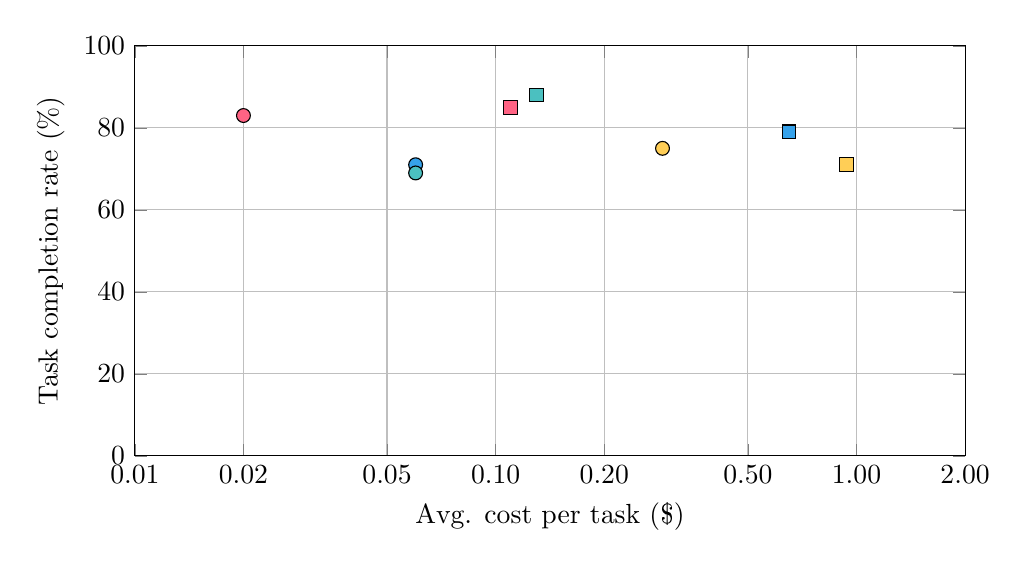
\begin{tikzpicture}
  \begin{axis}[
    width=\textwidth,
    height=0.56\textwidth,
    xmode=log,
    xmin=0.01, xmax=2,
    ymin=0, ymax=100,
    grid=both,
    xlabel={Avg. cost per task (\$)},
    xtick={0.01,0.02,0.05,0.1,0.2,0.5,1,2},
    xticklabels={$0.01$,$0.02$,$0.05$,$0.10$,$0.20$,$0.50$,$1.00$,$2.00$},
    minor x tick num=8,
    ylabel={Task completion rate (\%)},
  ]
    % BASIC tasks
    % RAG
    \addplot[only marks, mark=*, mark size=2.5pt, draw=black, fill=rag] coordinates {(0.02,83)};
    \addplot[only marks, mark=square*, mark size=2.5pt, draw=black, fill=rag] coordinates {(0.11,85)};
    % MCP
    \addplot[only marks, mark=*, mark size=2.5pt, draw=black, fill=mcp] coordinates {(0.06,71)};
    \addplot[only marks, mark=square*, mark size=2.5pt, draw=black, fill=mcp] coordinates {(0.65,79)};
    % NLWeb
    \addplot[only marks, mark=*, mark size=2.5pt, draw=black, fill=nlweb] coordinates {(0.06,69)};
    \addplot[only marks, mark=square*, mark size=2.5pt, draw=black, fill=nlweb] coordinates {(0.13,88)};
    % HTML
    \addplot[only marks, mark=*, mark size=2.5pt, draw=black, fill=htmlcol] coordinates {(0.29,75)};
    \addplot[only marks, mark=square*, mark size=2.5pt, draw=black, fill=htmlcol] coordinates {(0.94,71)};
  \end{axis}
\end{tikzpicture}
\caption{Basic tasks}
\end{subfigure}%
\makebox[0pt][l]{\hspace{-3cm}\begin{subfigure}{0.4\textwidth}
\centering
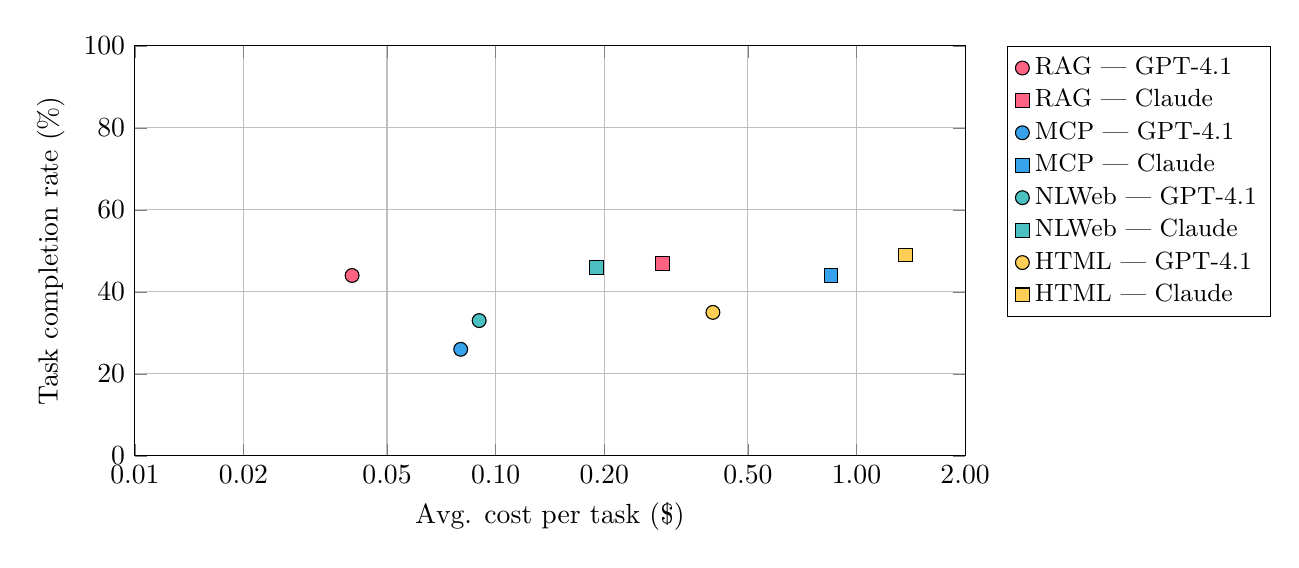
\begin{tikzpicture}
  \begin{axis}[
    width=\textwidth,
    height=0.56\textwidth,
    xmode=log,
    xmin=0.01, xmax=2,
    ymin=0, ymax=100,
    grid=both,
    xlabel={Avg. cost per task (\$)},
    xtick={0.01,0.02,0.05,0.1,0.2,0.5,1,2},
    xticklabels={$0.01$,$0.02$,$0.05$,$0.10$,$0.20$,$0.50$,$1.00$,$2.00$},
    minor x tick num=8,
    ylabel={Task completion rate (\%)},
    legend style={font=\small, at={(1.05,1)}, anchor=north west},
    legend cell align=left,
  ]
    % ADVANCED tasks
    % RAG
    \addplot[only marks, mark=*, mark size=2.5pt, draw=black, fill=rag] coordinates {(0.04,44)};
    \addplot[only marks, mark=square*, mark size=2.5pt, draw=black, fill=rag] coordinates {(0.29,47)};
    % MCP
    \addplot[only marks, mark=*, mark size=2.5pt, draw=black, fill=mcp] coordinates {(0.08,26)};
    \addplot[only marks, mark=square*, mark size=2.5pt, draw=black, fill=mcp] coordinates {(0.85,44)};
    % NLWeb
    \addplot[only marks, mark=*, mark size=2.5pt, draw=black, fill=nlweb] coordinates {(0.09,33)};
    \addplot[only marks, mark=square*, mark size=2.5pt, draw=black, fill=nlweb] coordinates {(0.19,46)};
    % HTML
    \addplot[only marks, mark=*, mark size=2.5pt, draw=black, fill=htmlcol] coordinates {(0.40,35)};
    \addplot[only marks, mark=square*, mark size=2.5pt, draw=black, fill=htmlcol] coordinates {(1.37,49)};
    
    % Shared legend
    \legend{
      RAG — GPT-4.1,
      RAG — Claude,
      MCP — GPT-4.1,
      MCP — Claude,
      NLWeb — GPT-4.1,
      NLWeb — Claude,
      HTML — GPT-4.1,
      HTML — Claude
    }
  \end{axis}
\end{tikzpicture}
\caption{Advanced tasks}
\end{subfigure}}

\caption{Cost vs. effectiveness for Basic (left) and Advanced (right) tasks. Color encodes interface (RAG, MCP, NLWeb, HTML). Shape encodes model (circle = GPT-4.1, square = Claude Sonnet 4).}
\label{fig:cost-vs-effectiveness-split}
\end{figure*}
